\PassOptionsToPackage{unicode=true}{hyperref} % options for packages loaded elsewhere
\PassOptionsToPackage{hyphens}{url}
%
\documentclass[]{article}
\usepackage{lmodern}
\usepackage{amssymb,amsmath}
\usepackage{ifxetex,ifluatex}
\usepackage{fixltx2e} % provides \textsubscript
\ifnum 0\ifxetex 1\fi\ifluatex 1\fi=0 % if pdftex
  \usepackage[T1]{fontenc}
  \usepackage[utf8]{inputenc}
  \usepackage{textcomp} % provides euro and other symbols
\else % if luatex or xelatex
  \usepackage{unicode-math}
  \defaultfontfeatures{Ligatures=TeX,Scale=MatchLowercase}
\fi
% use upquote if available, for straight quotes in verbatim environments
\IfFileExists{upquote.sty}{\usepackage{upquote}}{}
% use microtype if available
\IfFileExists{microtype.sty}{%
\usepackage[]{microtype}
\UseMicrotypeSet[protrusion]{basicmath} % disable protrusion for tt fonts
}{}
\IfFileExists{parskip.sty}{%
\usepackage{parskip}
}{% else
\setlength{\parindent}{0pt}
\setlength{\parskip}{6pt plus 2pt minus 1pt}
}
\usepackage{hyperref}
\hypersetup{
            pdftitle={Yumin Huang's CV},
            pdfauthor={Yumin Huang},
            pdfborder={0 0 0},
            breaklinks=true}
\urlstyle{same}  % don't use monospace font for urls
\usepackage[margin=1in]{geometry}
\usepackage{graphicx,grffile}
\makeatletter
\def\maxwidth{\ifdim\Gin@nat@width>\linewidth\linewidth\else\Gin@nat@width\fi}
\def\maxheight{\ifdim\Gin@nat@height>\textheight\textheight\else\Gin@nat@height\fi}
\makeatother
% Scale images if necessary, so that they will not overflow the page
% margins by default, and it is still possible to overwrite the defaults
% using explicit options in \includegraphics[width, height, ...]{}
\setkeys{Gin}{width=\maxwidth,height=\maxheight,keepaspectratio}
\setlength{\emergencystretch}{3em}  % prevent overfull lines
\providecommand{\tightlist}{%
  \setlength{\itemsep}{0pt}\setlength{\parskip}{0pt}}
\setcounter{secnumdepth}{0}
% Redefines (sub)paragraphs to behave more like sections
\ifx\paragraph\undefined\else
\let\oldparagraph\paragraph
\renewcommand{\paragraph}[1]{\oldparagraph{#1}\mbox{}}
\fi
\ifx\subparagraph\undefined\else
\let\oldsubparagraph\subparagraph
\renewcommand{\subparagraph}[1]{\oldsubparagraph{#1}\mbox{}}
\fi

% set default figure placement to htbp
\makeatletter
\def\fps@figure{htbp}
\makeatother


\title{Yumin Huang's CV}
\author{Yumin Huang}
\date{2021-10-24}

\begin{document}
\maketitle

\hypertarget{aside}{%
\section{Aside}\label{aside}}

\begin{figure}
\centering
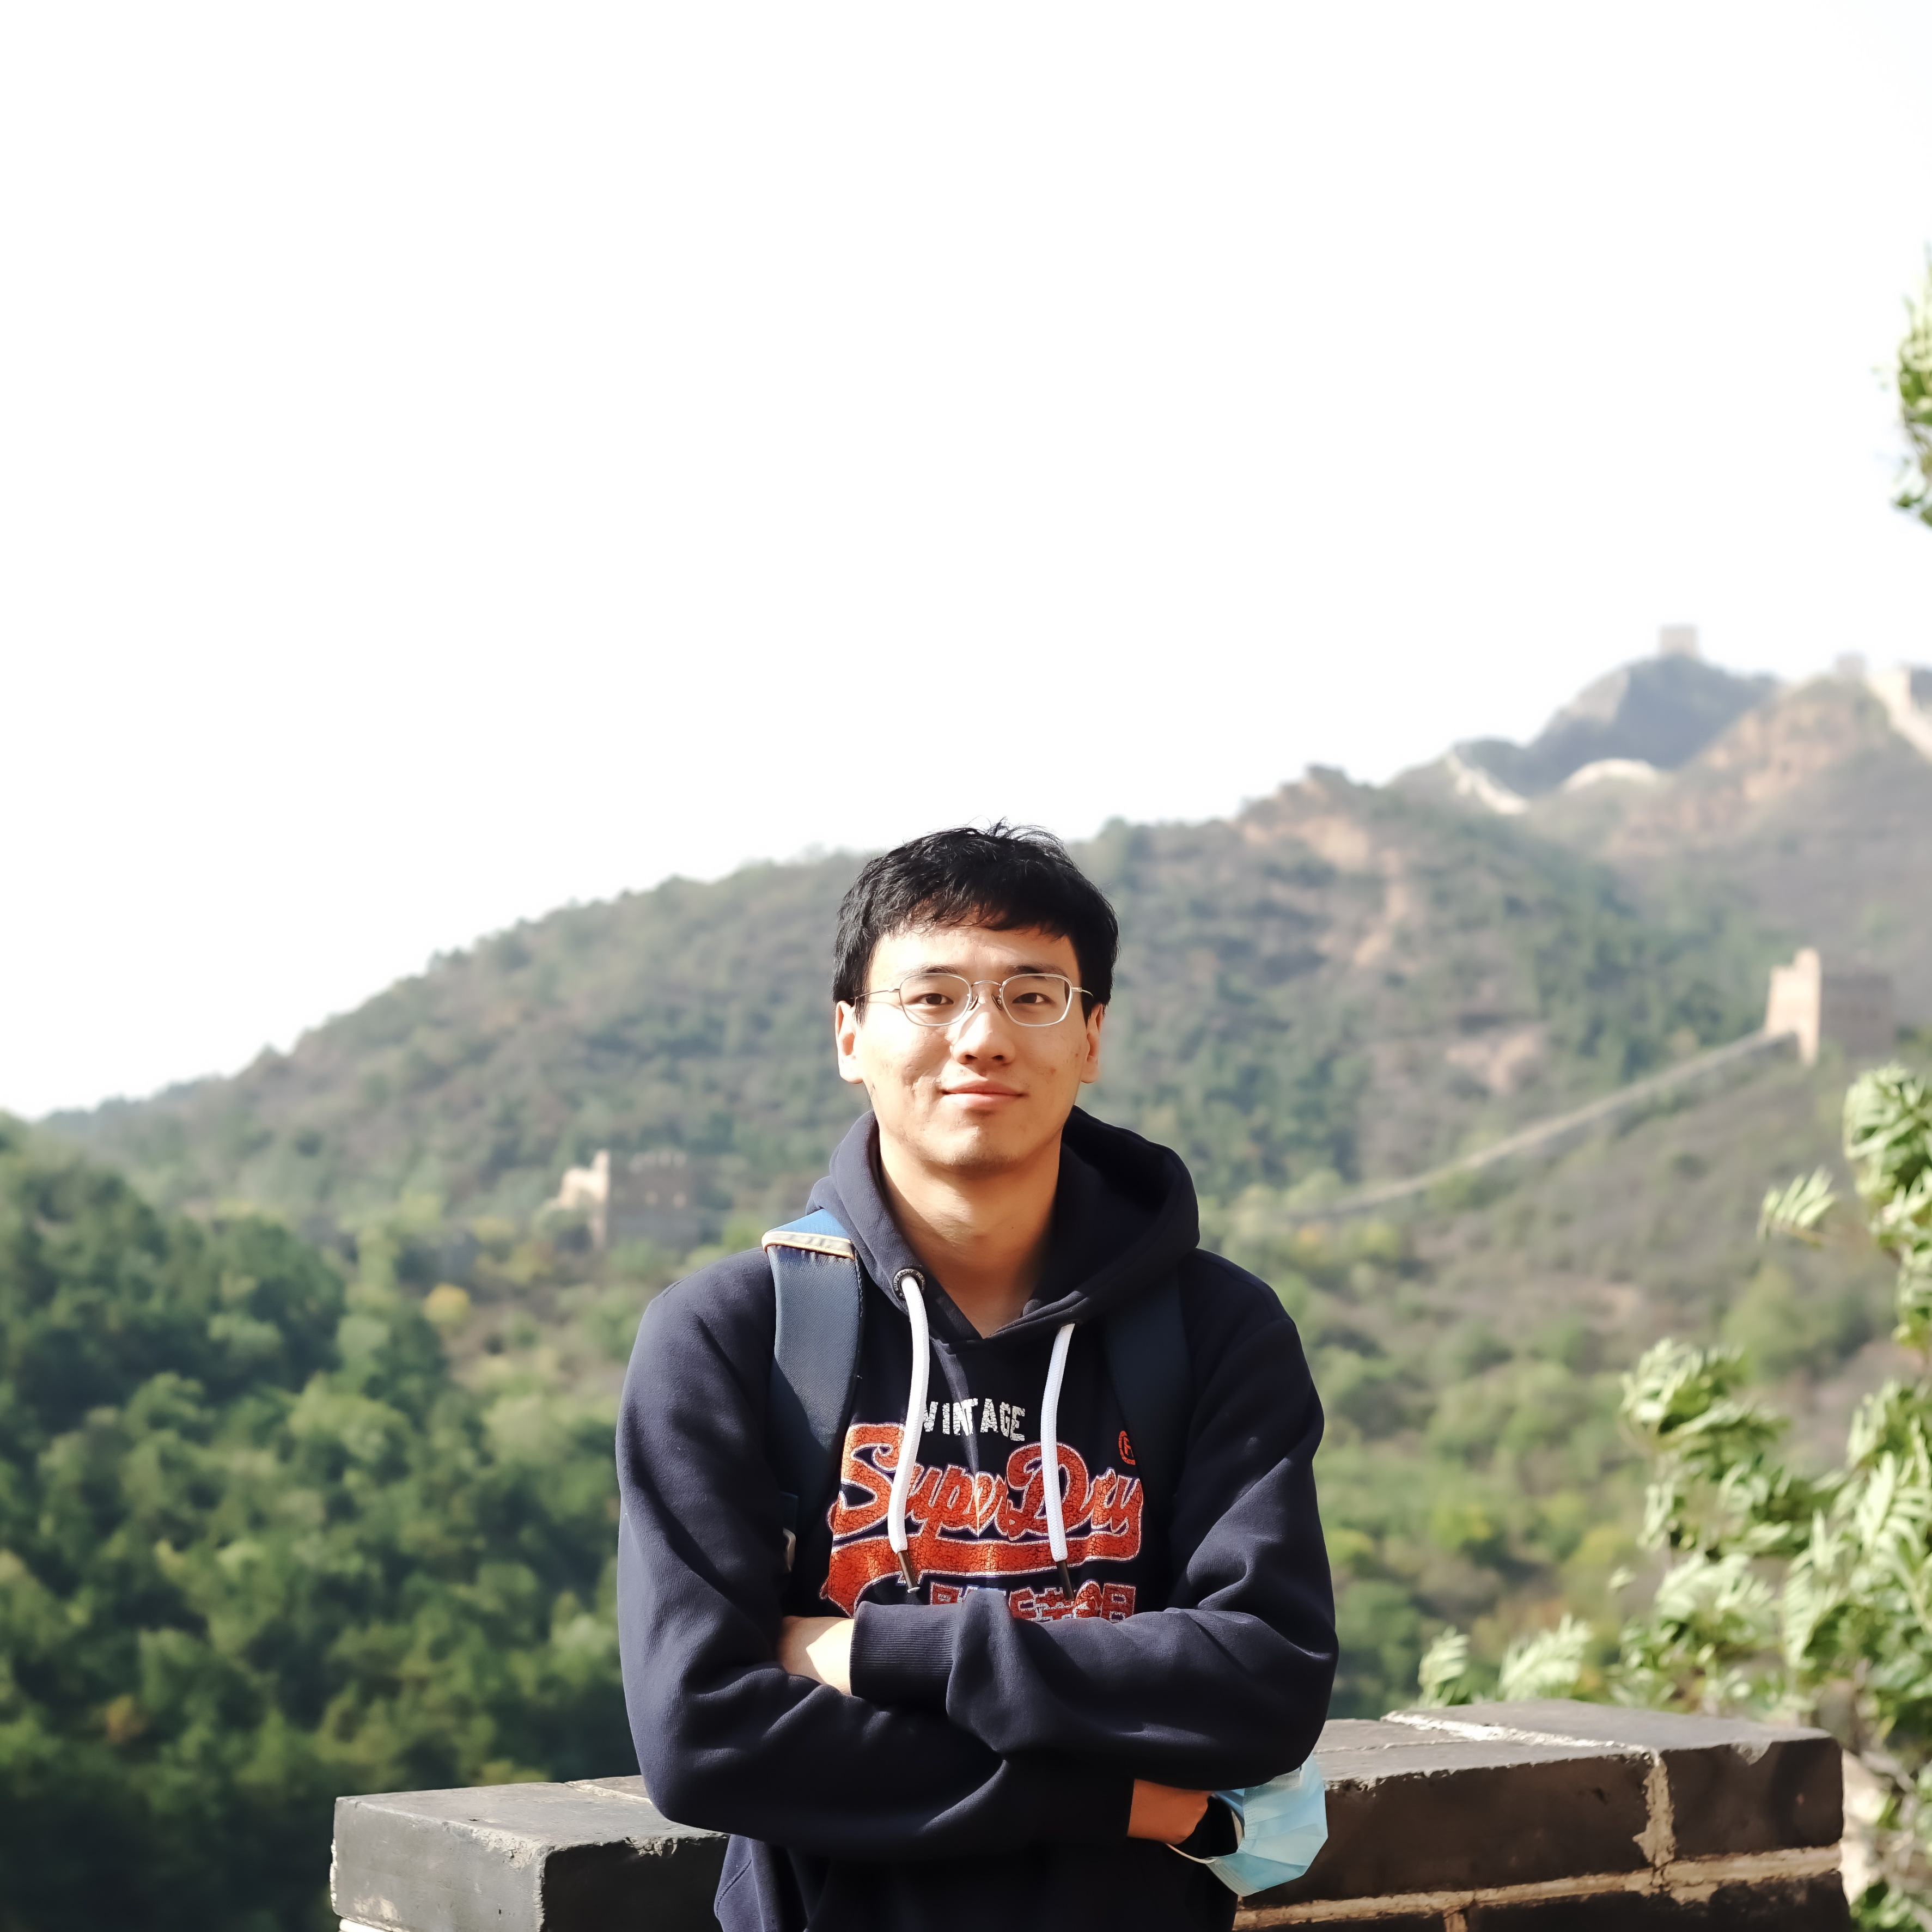
\includegraphics[width=1\textwidth,height=\textheight]{ymhuang.jpeg}
\caption{logo}
\end{figure}

View this CV online with links at \emph{sdws1983.github.io/cv}

\hypertarget{contact}{%
\subsection{Contact 联系方式}\label{contact}}

\begin{itemize}
\tightlist
\item
   \href{mailto:ymhuang@cau.edu.cn}{\nolinkurl{ymhuang@cau.edu.cn}}
\item
   \url{https://github.com/sdws1983}
\item
   \url{https://sdws1983.github.io/}
\item
   (86) 15652920371
\end{itemize}

\begin{itemize}
\tightlist
\item
  Citation = 47
\item
  H-index = 3
\item
  I10-index = 1
\end{itemize}

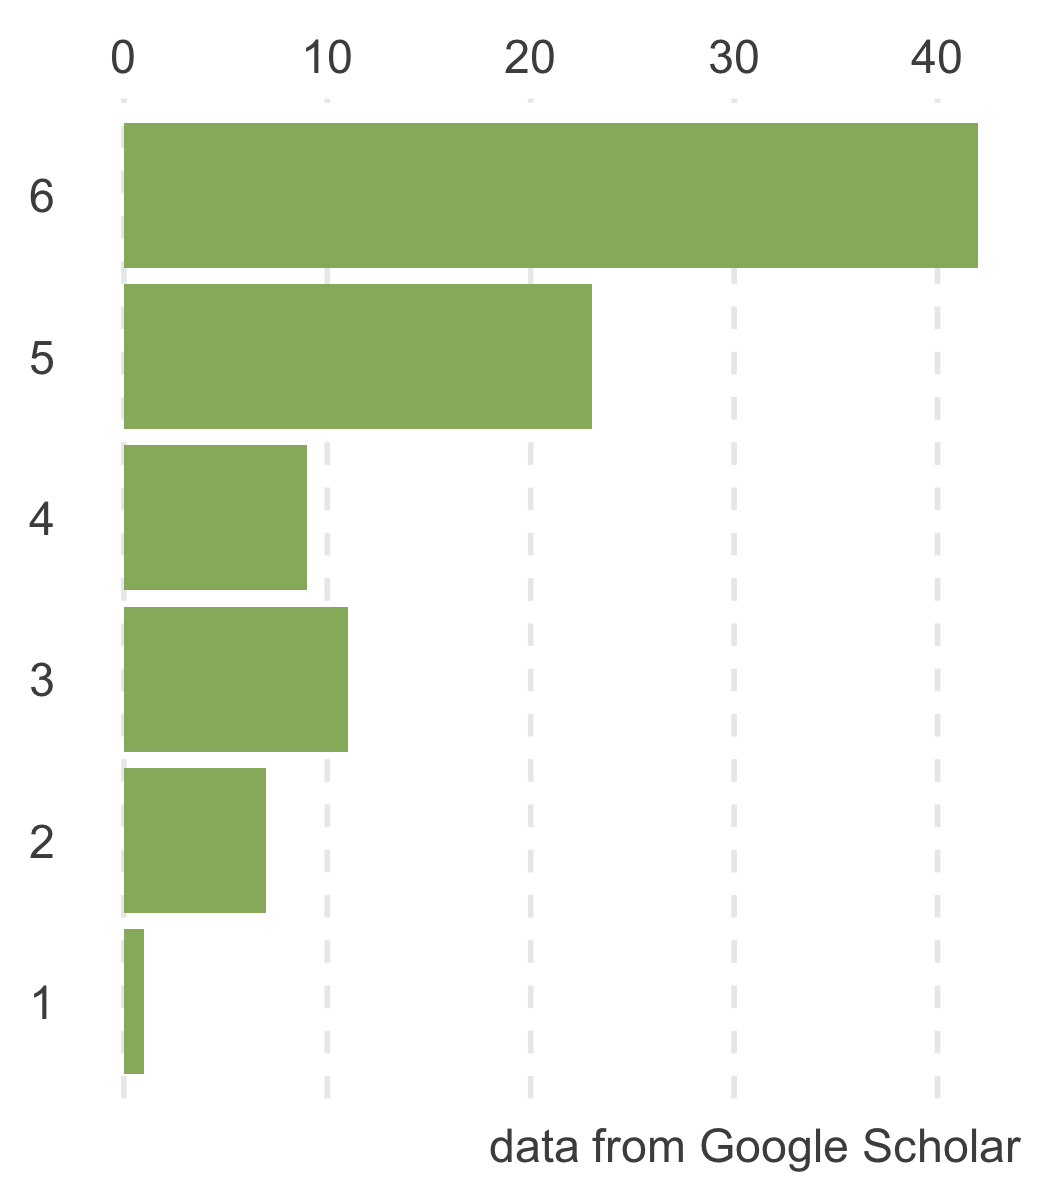
\includegraphics{citation.png}

\hypertarget{disclaimer}{%
\subsection{Disclaimer}\label{disclaimer}}

Last updated on 2021-10-24.

\hypertarget{main}{%
\section{Main}\label{main}}

\hypertarget{title}{%
\subsection{黄育敏 Yumin Huang}\label{title}}

PhD of Crop genetics and breeding at \href{http://www.cau.edu.cn/}{China
Agricultural University}.

中国农业大学,作物遗传育种专业博士.

I am broadly interested in comparative genomics, population genetics,
molecular evolution, epigenomics, 3D genomics, bioinformatics, data
integration and visualization.

本人对比较基因组学,群体遗传学,分子进化,表观遗传学,三维基因组学,生物信息学,数据处理及可视化等方面有着广泛兴趣。

\hypertarget{education-ux6559ux80b2ux7ecfux5386}{%
\subsection{Education
教育经历}\label{education-ux6559ux80b2ux7ecfux5386}}

\hypertarget{phd.-crop-genetics-and-breeding-ux4f5cux7269ux9057ux4f20ux80b2ux79cdux4e13ux4e1a-ux535aux58eb}{%
\subsubsection{PhD., Crop genetics and breeding 作物遗传育种专业,
博士}\label{phd.-crop-genetics-and-breeding-ux4f5cux7269ux9057ux4f20ux80b2ux79cdux4e13ux4e1a-ux535aux58eb}}

\href{http://cau.edu.cn/}{China Agricultural University} 中国农业大学

Beijing, CN

Present - 2016

\begin{itemize}
\tightlist
\item
  \href{http://maizecenter.cau.edu.cn/f}{国家玉米改良中心}
\item
  \href{http://sklppb.cau.edu.cn/}{植物生理学与生物化学国家重点实验室}
\item
  导师:金危危教授
\end{itemize}

\hypertarget{b.s.-biotechnology-ux751fux7269ux6280ux672fux4e13ux4e1a-ux5b66ux58eb}{%
\subsubsection{B.S., Biotechnology 生物技术专业,
学士}\label{b.s.-biotechnology-ux751fux7269ux6280ux672fux4e13ux4e1a-ux5b66ux58eb}}

\href{http://www.bjfu.edu.cn}{Beijing Forestry University} 北京林业大学

Beijing, CN

2016 - 2012

\begin{itemize}
\tightlist
\item
  \href{http://biology.bjfu.edu.cn/}{生物科学与技术学院}
\end{itemize}

\hypertarget{scholarships-awards-ux5956ux52b1ux8363ux8a89}{%
\subsection{Scholarships \& Awards
奖励荣誉}\label{scholarships-awards-ux5956ux52b1ux8363ux8a89}}

\hypertarget{ux535aux58ebux7814ux7a76ux751fux56fdux5bb6ux5956ux5b66ux91d1}{%
\subsubsection{博士研究生国家奖学金}\label{ux535aux58ebux7814ux7a76ux751fux56fdux5bb6ux5956ux5b66ux91d1}}

中华人民共和国教育部

N/A

2020

\hypertarget{ux5b66ux672fux6c47ux62a5ux4e8cux7b49ux5956}{%
\subsubsection{学术汇报二等奖}\label{ux5b66ux672fux6c47ux62a5ux4e8cux7b49ux5956}}

国家玉米改良中心年度论坛

N/A

\hypertarget{ux535aux58ebux4e00ux7b49ux5b66ux4e1aux5956ux5b66ux91d1}{%
\subsubsection{博士一等学业奖学金}\label{ux535aux58ebux4e00ux7b49ux5b66ux4e1aux5956ux5b66ux91d1}}

中国农业大学

N/A

2019

\hypertarget{ux535aux58ebux4e8cux7b49ux5b66ux4e1aux5956ux5b66ux91d1}{%
\subsubsection{博士二等学业奖学金}\label{ux535aux58ebux4e8cux7b49ux5b66ux4e1aux5956ux5b66ux91d1}}

中国农业大学

N/A

2018

\hypertarget{publications-ux53d1ux8868ux6587ux7ae0}{%
\subsection{Publications
发表文章}\label{publications-ux53d1ux8868ux6587ux7ae0}}

\hypertarget{megabase-scale-presence-absence-variation-with-tripsacum-origin-was-under-selection-during-maize-domestication-and-adaptation}{%
\subsubsection{\texorpdfstring{\href{https://doi.org/10.1186/s13059-021-02448-2}{Megabase-scale
presence-absence variation with \emph{Tripsacum} origin was under
selection during maize domestication and
adaptation}}{Megabase-scale presence-absence variation with Tripsacum origin was under selection during maize domestication and adaptation}}\label{megabase-scale-presence-absence-variation-with-tripsacum-origin-was-under-selection-during-maize-domestication-and-adaptation}}

\textbf{\emph{Genome Biology}}. 2021, 22(1):237. \textbf{(IF: 13.583,
JCR Q1)}

N/A

2021

\begin{itemize}
\tightlist
\item
  \textbf{Huang, Y.\textsuperscript{\#}}, Huang, W.\textsuperscript{\#},
  Meng, Z., Braz, G. T., Li, Y., Wang, K., Wang, H., Lai, J., Jiang, J.,
  Dong, Z.\textsuperscript{*}, \& Jin, W.\textsuperscript{*}
  \textbf{(第一作者)}
\end{itemize}

\hypertarget{evolution-and-domestication-footprints-uncovered-from-the-genomes-of-coix}{%
\subsubsection{\texorpdfstring{\href{http://dx.doi.org/10.1016/j.molp.2019.11.009}{Evolution
and Domestication Footprints Uncovered from the Genomes of
\emph{Coix}}}{Evolution and Domestication Footprints Uncovered from the Genomes of Coix}}\label{evolution-and-domestication-footprints-uncovered-from-the-genomes-of-coix}}

\textbf{\emph{Molecular Plant}}. 2019, 13(2):295-308. \textbf{(IF:
13.164, JCR Q1)}

N/A

2019

\begin{itemize}
\tightlist
\item
  Liu, H.\textsuperscript{\#}, Shi, J.\textsuperscript{\#}, Cai,
  Z.\textsuperscript{\#}, \textbf{Huang, Y.\textsuperscript{\#}}, Lv,
  M., Du, H., Gao, Q., Zuo, Y., Dong, Z., Huang, W., Qin, R., Liang, C.,
  Lai, J.\textsuperscript{*} , \& Jin, W.\textsuperscript{*}
  \textbf{(共同第一作者)}
\end{itemize}

\hypertarget{male-sterile-28-encodes-an-argonaute-family-protein-essential-for-male-fertility-in-maize}{%
\subsubsection{\texorpdfstring{\href{https://doi.org/10.1007/s10577-021-09653-6}{\emph{Male
sterile} 28 encodes an ARGONAUTE family protein essential for male
fertility in
maize}}{Male sterile 28 encodes an ARGONAUTE family protein essential for male fertility in maize}}\label{male-sterile-28-encodes-an-argonaute-family-protein-essential-for-male-fertility-in-maize}}

\textbf{\emph{Chromosome Research}}. 2021, 29(2):189-201 \textbf{(IF:
5.239, JCR Q2)}

N/A

2021

\begin{itemize}
\tightlist
\item
  Li, Y., \textbf{Huang, Y.}, Pan, L., Zhao, Y., Huang,
  W.\textsuperscript{*}, \& Jin, W.\textsuperscript{*}
\end{itemize}

\hypertarget{a-missense-mutation-in-a-large-subunit-of-ribonucleotide-reductase-confers-temperature-gated-tassel-formation}{%
\subsubsection{\texorpdfstring{\href{https://doi.org/10.1104/pp.20.00219}{A
missense mutation in a large subunit of ribonucleotide reductase confers
temperature-gated tassel
formation}}{A missense mutation in a large subunit of ribonucleotide reductase confers temperature-gated tassel formation}}\label{a-missense-mutation-in-a-large-subunit-of-ribonucleotide-reductase-confers-temperature-gated-tassel-formation}}

\textbf{\emph{Plant Physiology}}. 2020, 184(4):1979-1997 \textbf{(IF:
8.34, JCR Q1)}

N/A

2020

\begin{itemize}
\tightlist
\item
  Xie, S.\textsuperscript{\#}, Luo, H.\textsuperscript{\#},
  \textbf{Huang, Y.}, Wang, Y., Ru, W., Shi, Y., Huang, W., Wang, H.,
  Dong, Z., \& Jin, W.\textsuperscript{*}
\end{itemize}

\hypertarget{dlf1-promotes-floral-transition-by-directly-activating-zmmads4-and-zmmads67-in-the-maize-shoot-apex}{%
\subsubsection{\texorpdfstring{\href{https://dx.doi.org/10.1111/nph.16772}{\emph{dlf1}
promotes floral transition by directly activating \emph{ZmMADS4} and
\emph{ZmMADS67} in the maize shoot
apex}}{dlf1 promotes floral transition by directly activating ZmMADS4 and ZmMADS67 in the maize shoot apex}}\label{dlf1-promotes-floral-transition-by-directly-activating-zmmads4-and-zmmads67-in-the-maize-shoot-apex}}

\textbf{\emph{New Phytologist}}. 2020, 228(4):1386-1400. \textbf{(IF:
10.151, JCR Q1)}

N/A

\begin{itemize}
\tightlist
\item
  Sun, H.\textsuperscript{\#}, Wang, C.\textsuperscript{\#}, Chen, X.,
  Liu, H., \textbf{Huang, Y.}, Li, S., Dong, Z., Zhao, X., Tian,
  F.\textsuperscript{*}, \& Jin, W.\textsuperscript{*}
\end{itemize}

\hypertarget{maize-male-sterile-33-encodes-a-putative-glycerol-3-phosphate-acyltransferase-that-mediates-anther-cuticle-formation-and-microspore-development}{%
\subsubsection{\texorpdfstring{\href{https://doi.org/10.1186/s12870-018-1543-7}{Maize
\emph{male sterile 33} encodes a putative glycerol-3-phosphate
acyltransferase that mediates anther cuticle formation and microspore
development}}{Maize male sterile 33 encodes a putative glycerol-3-phosphate acyltransferase that mediates anther cuticle formation and microspore development}}\label{maize-male-sterile-33-encodes-a-putative-glycerol-3-phosphate-acyltransferase-that-mediates-anther-cuticle-formation-and-microspore-development}}

\textbf{\emph{BMC Plant Biology}}. 2018, 18(1). \textbf{(IF: 4.215, JCR
Q1)}

N/A

2018

\begin{itemize}
\tightlist
\item
  Zhang, L.\textsuperscript{\#}, Luo, H.\textsuperscript{\#}, Zhao,
  Y.\textsuperscript{\#}, Chen, X., \textbf{Huang, Y.}, Yan, S., Li, S.,
  Liu, M., Huang, W., Zhang, X., \& Jin, W.\textsuperscript{*}
\end{itemize}

\hypertarget{leaf-extract-from-lithocarpus-polystachyus-rehd.-promote-glycogen-synthesis-in-t2dm-mice}{%
\subsubsection{\texorpdfstring{\href{https://dx.doi.org/10.1371/journal.pone.0166557}{Leaf
extract from \emph{Lithocarpus polystachyus} Rehd. Promote glycogen
synthesis in T2DM
mice}}{Leaf extract from Lithocarpus polystachyus Rehd. Promote glycogen synthesis in T2DM mice}}\label{leaf-extract-from-lithocarpus-polystachyus-rehd.-promote-glycogen-synthesis-in-t2dm-mice}}

\textbf{\emph{PLoS ONE}}. 2016, 11(11). \textbf{(IF: 3.240, JCR Q2)}

N/A

2016

\begin{itemize}
\tightlist
\item
  Wang, J.\textsuperscript{\#}, \textbf{Huang, Y.\textsuperscript{\#}},
  Li, K.\textsuperscript{\#}, Chen, Y., Vanegas, D., McLamore, E. S., \&
  Shen, Y.*\textsuperscript{*} \textbf{(共同第一作者)}
\end{itemize}

\hypertarget{research-experience-ux7814ux7a76ux7ecfux5386}{%
\subsection{Research Experience
研究经历}\label{research-experience-ux7814ux7a76ux7ecfux5386}}

\hypertarget{ux7389ux7c73ux57faux56e0ux7ec4ux4e2dux5927ux7247ux6bb5ux7f3aux5931ux53d8ux5f02ux7684ux52a8ux6001ux6f14ux5316ux7814ux7a76}{%
\subsubsection{玉米基因组中大片段缺失变异的动态演化研究}\label{ux7389ux7c73ux57faux56e0ux7ec4ux4e2dux5927ux7247ux6bb5ux7f3aux5931ux53d8ux5f02ux7684ux52a8ux6001ux6f14ux5316ux7814ux7a76}}

主导

N/A

2021 - 2018

\begin{itemize}
\tightlist
\item
  独立完成该课题的所有基因组学分析,参与设计了该课题的研究思路及技术路线,与通讯作者共同完成了文章撰写及同行评议。
\item
  通过整合细胞遗传学、基因组组装、群体遗传学、系统发育学以及进化比较等多种手段实现了一项创新性的跨学科研究。
\item
  在国际知名基因组学期刊《Genome
  Biology》发表研究论文一篇,获得海内外同行的广泛关注及积极评价。\textbf{解析了基因组进化和物种形成过程中``化石''结构变异的动态进化和功能,为玉米物种形成、驯化进程等理论研究以及基因组结构变异遗传资源在育种中的应用提供了新的思路。}
\end{itemize}

\hypertarget{ux7389ux7c73ux5168ux57faux56e0ux7ec4ux4e2dux5f00ux653eux67d3ux8272ux8d28ux7684ux9057ux4f20ux548cux91cdux5851}{%
\subsubsection{玉米全基因组中开放染色质的遗传和重塑}\label{ux7389ux7c73ux5168ux57faux56e0ux7ec4ux4e2dux5f00ux653eux67d3ux8272ux8d28ux7684ux9057ux4f20ux548cux91cdux5851}}

主导

N/A

Present - 2020

\begin{itemize}
\tightlist
\item
  独立完成该课题的所有基因组学分析,参与设计了该课题的研究思路及技术路线。
\item
  设计开发了一套跨基因组比较分析流程,探究开放染色质与玉米杂种优势的关联。
\item
  主要基因组学结果基本完成,文章手稿准备中。
\end{itemize}

\hypertarget{ux858fux82e1ux57faux56e0ux7ec4ux7ec4ux88c5ux6ce8ux91caux5206ux6790}{%
\subsubsection{薏苡基因组组装注释分析}\label{ux858fux82e1ux57faux56e0ux7ec4ux7ec4ux88c5ux6ce8ux91caux5206ux6790}}

参与主导

N/A

2019 - 2016

\begin{itemize}
\tightlist
\item
  合作完成该课题的部分基因组学分析及分子实验,参与设计了该课题的研究思路以及技术路线,参与完成了文章撰写及同行评议。
\item
  主要负责物种树的构建、基因家族分析、薏苡GBS群体数据分析、遗传图谱的构建及以薏苡转录组的比较分析,参与了薏苡群体测序材料的收集和构建。
\item
  在国际知名植物领域期刊《Molecular
  Plant》发表研究论文一篇,\textbf{发布了世界上首个薏苡基因组参考序列,揭示了薏苡的进化及驯化足迹。}
\end{itemize}

\hypertarget{ux5b9eux9a8cux5ba4ux516cux5171ux6570ux636eux5206ux6790}{%
\subsubsection{实验室公共数据分析}\label{ux5b9eux9a8cux5ba4ux516cux5171ux6570ux636eux5206ux6790}}

参与

N/A

Present - 2016

\begin{itemize}
\tightlist
\item
  帮助实现实验室其他成员的生物信息学分析需求。
\item
  实施RNA-seq, ChIP-seq, ATAC-seq,
  BSA-seq等一些测序数据的分析,基因序列比较分析,群体遗传学分析,驯化位点挖掘。
\item
  参与了实验室其他一些文章的发表。
\end{itemize}

\hypertarget{ux5b9eux9a8cux5ba4ux751fux7269ux4fe1ux606fux5b66ux8d44ux6e90ux7684ux7ef4ux62a4ux7ba1ux7406}{%
\subsubsection{实验室生物信息学资源的维护管理}\label{ux5b9eux9a8cux5ba4ux751fux7269ux4fe1ux606fux5b66ux8d44ux6e90ux7684ux7ef4ux62a4ux7ba1ux7406}}

负责人

N/A

\begin{itemize}
\tightlist
\item
  实验室计算服务器的管理维护,公共数据的备份,测序相关事宜的沟通。
\item
  独立搭建并维护实验室网站,开发了一些网页工具服务于实验室成员科研日常。
\end{itemize}

\hypertarget{conference-attendance-ux5b66ux672fux6d3bux52a8}{%
\subsection{Conference attendance
学术活动}\label{conference-attendance-ux5b66ux672fux6d3bux52a8}}

\hypertarget{chinese-genomics-meet-up-online-cgm-ux534eux4ebaux57faux56e0ux7ec4ux5b66ux5728ux7ebfux6c99ux9f99}{%
\subsubsection{\texorpdfstring{\href{https://cgmonline.co/}{Chinese
Genomics Meet-up online (CGM)
华人基因组学在线沙龙}}{Chinese Genomics Meet-up online (CGM) 华人基因组学在线沙龙}}\label{chinese-genomics-meet-up-online-cgm-ux534eux4ebaux57faux56e0ux7ec4ux5b66ux5728ux7ebfux6c99ux9f99}}

\href{https://www.bilibili.com/video/BV1a44y147A5}{Invited talks}
特邀报告

Virtual Conference

2021

\hypertarget{the-63rd-annual-maize-genetics-meeting-ux7b2c63ux5c4aux7389ux7c73ux9057ux4f20ux5b66ux5e74ux5ea6ux4f1aux8bae}{%
\subsubsection{\texorpdfstring{\href{https://www.maizegdb.org/mgc/maizemeeting/2021/}{The
63rd Annual Maize Genetics Meeting
第63届玉米遗传学年度会议}}{The 63rd Annual Maize Genetics Meeting 第63届玉米遗传学年度会议}}\label{the-63rd-annual-maize-genetics-meeting-ux7b2c63ux5c4aux7389ux7c73ux9057ux4f20ux5b66ux5e74ux5ea6ux4f1aux8bae}}

Poster presentation 墙报展示

Virtual Conference

\hypertarget{ux7b2cux4e00ux5c4aux5168ux56fdux4f5cux7269ux5b66ux79d1ux535aux58ebux540eux5b66ux672fux8bbaux575b}{%
\subsubsection{\texorpdfstring{\href{http://ncpd.cau.edu.cn/}{第一届全国作物学科博士后学术论坛}}{第一届全国作物学科博士后学术论坛}}\label{ux7b2cux4e00ux5c4aux5168ux56fdux4f5cux7269ux5b66ux79d1ux535aux58ebux540eux5b66ux672fux8bbaux575b}}

参会

海南三亚

2020

\hypertarget{ux4e2dux56fdux519cux4e1aux5927ux5b66ux519cux5b66ux96622020ux5e74ux5ea6ux535aux58ebux751fux8bbaux575b}{%
\subsubsection{\texorpdfstring{\href{http://cab.cau.edu.cn/art/2020/10/16/art_23547_711508.html}{中国农业大学农学院2020年度博士生论坛}}{中国农业大学农学院2020年度博士生论坛}}\label{ux4e2dux56fdux519cux4e1aux5927ux5b66ux519cux5b66ux96622020ux5e74ux5ea6ux535aux58ebux751fux8bbaux575b}}

报告

北京

\hypertarget{ux5e74ux56fdux5bb6ux7389ux7c73ux6539ux826fux4e2dux5fc3ux7814ux7a76ux751fux5b66ux672fux8bbaux575b}{%
\subsubsection{\texorpdfstring{\href{http://maizecenter.cau.edu.cn/f/view-4-8481b7bf0f8347509a67269db87ca087.html}{2020年国家玉米改良中心研究生学术论坛}}{2020年国家玉米改良中心研究生学术论坛}}\label{ux5e74ux56fdux5bb6ux7389ux7c73ux6539ux826fux4e2dux5fc3ux7814ux7a76ux751fux5b66ux672fux8bbaux575b}}

报告

北京

\hypertarget{ux7b2cux56dbux5c4aux5168ux56fdux7389ux7c73ux751fux7269ux5b66ux5b66ux672fux7814ux8ba8ux4f1a}{%
\subsubsection{\texorpdfstring{\href{http://www.maizemeeting.org/2019/}{第四届全国玉米生物学学术研讨会}}{第四届全国玉米生物学学术研讨会}}\label{ux7b2cux56dbux5c4aux5168ux56fdux7389ux7c73ux751fux7269ux5b66ux5b66ux672fux7814ux8ba8ux4f1a}}

参会

河南郑州

2019

\hypertarget{ux7b2cux4e09ux5c4aux5168ux56fdux7389ux7c73ux751fux7269ux5b66ux5b66ux672fux7814ux8ba8ux4f1a}{%
\subsubsection{\texorpdfstring{\href{http://www.maizemeeting.org/2018/}{第三届全国玉米生物学学术研讨会}}{第三届全国玉米生物学学术研讨会}}\label{ux7b2cux4e09ux5c4aux5168ux56fdux7389ux7c73ux751fux7269ux5b66ux5b66ux672fux7814ux8ba8ux4f1a}}

参会

山东青岛

2018

\end{document}
